		\chapter{Blender Animation}
        	\index{animating}
            \index{animation}
			Before even acquiring the \index{hexapod}hexapod, I had formulated the idea that to easily create any form of dancing hexapod, you'd need some sort of 3D animation software.\\				
         	\textit{\textbf{Also See: }\hyperref[manual_blender]{BaralabaBob Technical Manual: Blender}}
            
			After acquiring the \index{hexapod}hexapod, and started \index{programming}programming it - I once again reaffirmed the need for this software.\\
			
            \index{Blender}
			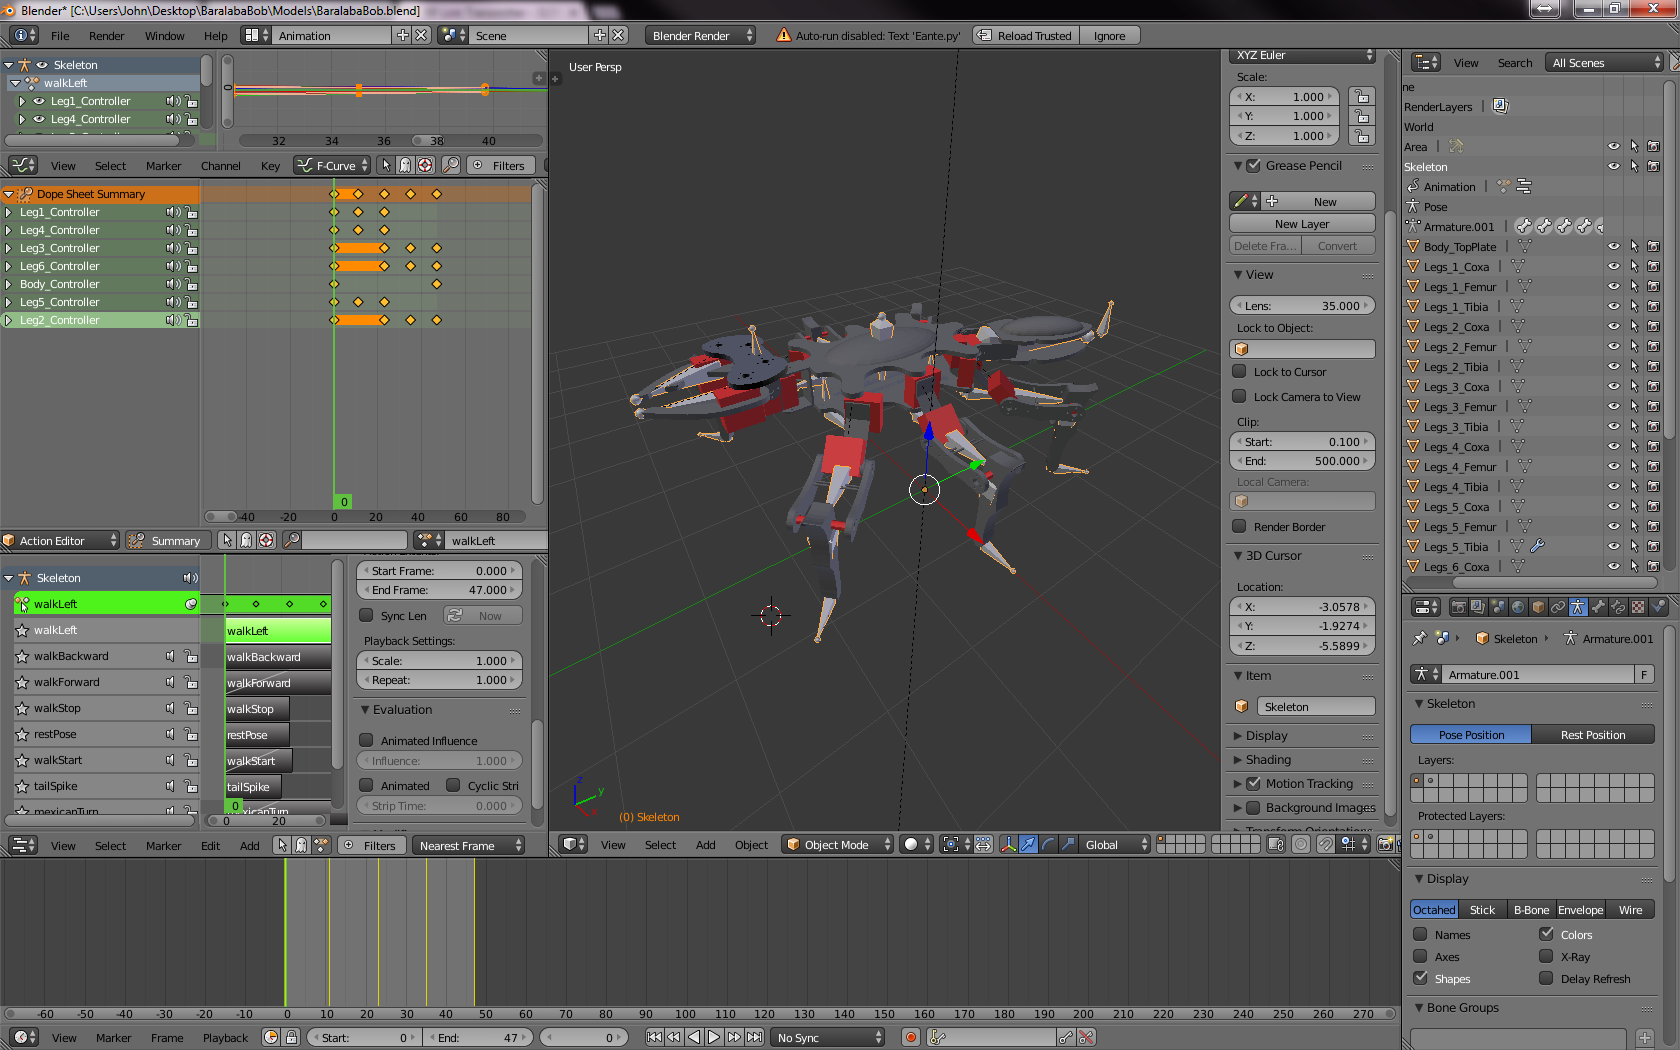
\includegraphics[width=\linewidth]{images/blender}
			
			\section{Base Software Choice}
            	\index{animation}
				Writing 3D animation software from scratch would be reinventing the wheel - so I looked for an existing \index{3D}3D \index{modeling}modeling and animation program that I could use as the "base software" for this idea.\\
				
				The two best options where Maya and Blender. Both of which support \index{python}\index{scripting}python scripting, and can be downloaded freely as a \index{student}student.\\
				
				I ended up choosing Blender for many reasons, a few of which listed are listed in the following: it being much smaller in \index{file size}file size, \index{open source}open source nature, and being written in \index{python}python.\\
				
			\section{Model}
				I needed a scale model of the hexapod in a digital form to animate in Blender. A model was created in \index{TurboCAD} TurboCAD 2011 to scale, and exported in the \index{3DS}3DS format to \index{blender}Blender.\\
				
				After being colored appropriately, I added an armature to the model that correctly mimics the \index{joints}joints in the actual robot. The model is attached to this armature - as I move and animate the \index{armature}armature, the model also follows.\\			
			
			\section{Scripting}
				After animating the model, I needed to export that data to a form that the \index{hexapod}hexapod can playback. This is where blender's \index{scripting}scriptability comes in.\\
				
				I first attempted to write a script that would extract the armature data when told in the standard blender interface. Unfortunately for some reason I couldn't achieve this (I forget why...). Instead the script, named \index{Eante}Eante (pronounced Yaantay), cycles through the selected action and records all the important \index{keyframes}keyframes.\\
				
				Eante then saves this information in \index{compiler}compiler\_config.dat, ready for the next script, Dumper.py.\\
				
				I found that I was able to easily read the armature information in \index{Blender}Blender's Game Engine mode. As such I wrote a script that would open the compiler\_config.dat, playback the selected animation, and then record any changed joint positions at the specified keyframes.\\
				
				Dumper saves this information in a .act file. I then manually copy the contents of this information to the actions folder on the \index{hexapod}hexapod. In the future this will happen automatically.\\
				
            
            \index{bezier}
            \index{linear}
			\section{Linear \& Bezier Modes}
				Outlined above (where the system only captures bone positions on relevant keyframes) is considered Linear mode. When playing back on the robot, the movements aren't very smooth - there is a constant speed on each movement, and no sort of ramping.\\
				
				When creating keyframes, blender automatically interpolates the position of keyframed objects between frames with a cubic bezier curve speed modifier.\\
				
				So in the animation you would see very nice smooth ramping, whereas on the robot the movements would look very, well, robotic and stiff. \\
				
				At this point I decided to create "bezier mode". When Eante compiled the keyframes to check, it would present the option for bezier mode. If you selected bezier mode it would write said setting to compiler\_config.dat. When Dumper reads that bezier mode is enabled, it ignores all keyframe data, and simply saves the armature angles every 3 frames (this is configurable, of course).\\
				
				The idea of this was that the robot would have smoother movements. The concept was sound, but execution had a few issues. Firstly I hadn't properly implemented timing.\\
				
				If you think about it, when a .act files specifies the angle of a joint at a certain frame - the joint has to be at that position by the time that frame has been reached. Instead, I told the joints to reach their positions by the next frame - wreaking havoc within the bezier system.\\
				
				I created some systems to counter this, the result was some very smooth movements, but timing accuracy suffered.\\
				
				Since then I have fixed the timing implementation, and the bezier mode works perfectly now, creating incredibly smooth movements. An alternative was considered where I implement the bezier curve calculations within the processor on the fly. That way, you save the amount of file each action takes up, by only storing keyframe data, and \index{interpolation}\index{interpolating}interpolating positions to a function of a bezier curve manually. This is on the TODO list, however due to fixing the timing issue, I may not deem it worth my while to implement it.\\